%Name: Template of COMP9020 Assignments
%Author:Jack
%Date: 14/08/2017
%Acknowledgement: This template is based on work of Brendan Trinh of UNSW MathSoc 2015
\documentclass[11pt, a4paper]{article}

\usepackage{amsmath} % Improves structure of typed out maths
\usepackage{mathtools} % Improves upon deficiencies of amsmath package
\usepackage{amssymb} % Adds some handy symbols to use.
\usepackage{amsthm} % Adds some neat formulas to use, e.g. \begin{proof} etc.

\usepackage[a4paper]{geometry} % Default page margins can be altered.
\usepackage{microtype} % Improves spacing between letters.
\usepackage{booktabs} % Improves tables. Can now create without vertical separators.
\usepackage{array} % Includes more options for arrays
\usepackage{paralist} % More flexible use of itemize, enumerate, etc.
\usepackage{graphicx} % Add images to your document
\usepackage{color} % Allows for the use of colours!
\usepackage{cleveref} % Better cross-referencing
\usepackage{hyperref} % For adding hyperlinks
\usepackage{fancyhdr} % Customise headers & footers in document
\usepackage{paralist}

\usepackage{url} % For adding url

\begin{document}
\title{COMP9020 - Assignment 2}
\author{Jack Jiang (z5129432)}
\date{ 24 September 2017 }
\maketitle
\graphicspath{{Graphics/}}

\section*{Question 1}
\begin{enumerate}[(a)]
    \item
    For graph G = (E, V) as follows:
    \begin{center}
        \includegraphics{q1a1}
    \end{center}
    For every $e = (v, w) \in E$
    $$ c(v) \ne c(w) $$
    The mininum number of colors to sufficient effect such a mapping, denoted:
    $$ \chi(G) $$
    \item
    The minimum number of colors is 2, as follows:
    \begin{center}
        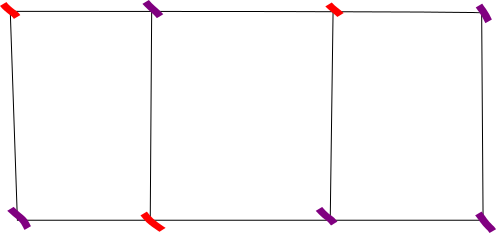
\includegraphics[scale=0.7]{q1b1}
    \end{center}
    \item
    The connection of the graph changes, as follows:
    \begin{center}
        \includegraphics[scale=0.7]{q1c1}
    \end{center}
    Because v2 connect to v3, so they must be different colours, $c(v2) \ne c(v3)$
    v2 and v3 connect to all other vertex, so other vertex must use different colours other than c(v2) and c(v3)
    $$c(v1) \ne c(v2) \ne c(v3)$$
    also, v1 connect to v4, so $c(v1) \ne c(v4)$, at lease we should use 4 different colors
    Because I can use 4 different colors as shows in graph, therefore:
    $$ \chi(G) = 4 $$
\end{enumerate}

\section*{Question 2}
\begin{enumerate}[(a)]
    \item
    \{A$_v$ :  $ \sum_{c \in C} P_{v, c}$\}
    \item
    \{B$_v$ :  $ \forall c,d \in C, \neg (P_{v, c} \land P_{v, d})$\}
    \item
    \{C$_{u, v}$ :  $ \forall c \in C, \neg (P_{v, c} \land P_{u, c})$\}
    \item
    \{$\varphi_G$ :  $ \forall (u,v) \in E $, $\neg (P_{v, c} \land P_{u, c})$ and $ \forall c,d,e \in C$, $\sum_{v \in V}(P_{v, c} \lor P_{v, d} \lor P_{v, e})$ \}
\end{enumerate}

\section*{Question 3}
\begin{enumerate}[(a)]
    \item
    (R):
    $$ x \lor x = x \implies x \sqsubseteq x \,  for\, all\, x \in S $$
    (AS):
    $$ x \sqsubseteq y \implies x \lor y = y $$
    $$ y \sqsubseteq x \implies y \lor x = x $$
    $$ \because x \lor y =y \lor x$$
    $$ \therefore x =y $$
    (T):
    $$ x \sqsubseteq y \implies x \lor y = y $$
    $$ y \sqsubseteq z \implies y \lor z = z $$
    $$ x \lor z = x \lor (y \lor z) = (x \ lor y) \lor z = y \lor z = z $$
    $$ \therefore x \sqsubseteq z $$
    (L): not satisfied\\
    for x, y are not empty, if x $\lor y = \emptyset $, then:\\
    neither $x \sqsubseteq y$, nor $ y \sqsubseteq x $
    \item
    $ \sqsubseteq $ is corresponse to $ \subseteq $
    $$ x \subseteq y \iff x \cup y = y $$
    \item
    Draw a trueth table:\\
    \begin{tabular}{ | c | c | c | c |}
        \hline
        x & y & $x \lor y$ & $ (x \lor y ) \rightleftarrows y$\\
        \hline
        T & T & T & T\\
        \hline
        T & F & T & F\\
        \hline
        F & T & T & T\\
        \hline
        F & F & F & T\\
        \hline
        \end{tabular}\\
        Therefore, the logic equivilence is:
        $$ xy + \bar{x}y + \overline{xy} = y + \overline{xy}$$
\end{enumerate}

\section*{Question 4}
\begin{enumerate}[(a)]
    \item
    assume that add(0, n) = n\\
    for n=0, add(0, 0) = 0\\
    for n$>$0, add(0, n+1) = add(0, n) + 1 = n + 1\\
    therefore,for n $\in$ N,\\
    add(0, n) = n\\
    because add(n, 0) = n\\
    therefore, P(n) holds for all n $\in$ N
    \item
    a + b = n $\implies$ b = n - a\\
    assume that add(a, n-a) = n\\
    for n=a, add(a, n-a) = add(a, 0) + 0 = a = n\\
    for n$\>$a, add(a, n-a+1) = add(a, n-a) + 1 = n + 1\\
    therefore, add(a, n-a) = n\\
    follow similar steps, we can prove that:\\
    add(b, n-b) = n\\
    Therefore add(a, b) = add(b, a) = a + b = n
\end{enumerate}

\section*{Question 5}
\begin{enumerate}[(a)]
    \item
    $rec\_a(n):$\\
    $if n<2: return\, n$\\
    $else:$\\
        $x:=rec_a(n-1) --> T(n-1)$\\
        $y:=rec_a(n-2) --> T(n-2)$\\
        $return 5x-6y --> 1$\\
    The total cost is $T(n-1)+T(n-2)+1$\\
    $T(1)=0$\\
    $T(2)=0$\\
    $T(n)=T(n-1)+T(n-2)+1$\\
    Where $T(n+1)$ is a fibonacci number\\
    according to Binet's Formula$(http://mathworld.wolfram.com/BinetsFibonacciNumberFormula.html)$\\
    $T(n+1) = \frac{\phi^n-(-\phi^{-n})}{\sqrt{5}}$\\
    where $\phi$ is golden ratio\\
    therefore the upper bound for $rec\_a(n)$ is $\phi^n$
    where $\phi=1.618$
    \\
    $iter\_a(n):$\\
    $if n<2: return\, n$\\
    $else:$\\
    $x:=1$\\
    $y:=0$\\
    $i:=1 --> 3$\\
    $while i<n:$\\
    $i:=x$\\
    $x:=5x-6y$\\
    $y:=t$\\
    $i:=i+1 --> 4n$\\
    $return\, x$\\
    The total cost is $4n+4$\\
    The upper bound for $iter\_a(n)$ is n
    \item
    draw a table\\
    \begin{tabular}{ | c | c | c | }
        \hline
        n & $a_n$ & $ a_n+2^n $ \\
        \hline
        0 & 0 & 1\\
        \hline
        1 & 1 & 3\\
        \hline
        2 & 5 & 9\\
        \hline
        3 & 19 & 27\\
        \hline
        4 & 65 & 81\\
        \hline
        5 & 211 & 243\\
        \hline
        6 & 665 & 729\\
        \hline
        7 & 2059 & 2187\\
        \hline
    \end{tabular}\\
    Guess $a_n=3^n-2^n$\\
    for n = 0, $a_n=0$ holds\\
    for n = 1, $a_n=3-2=1$ holds\\
    assume $a_n=3^n-2^n$ holds for some n $>$ 1\\
    $a_n = 5*a_{n-1} - 6a_{n-2}$\\
    $= 5*(3^{n-1}-2^{n-1}) - 6*(3^{n-2}-2^{n-2})$\\
    $= 5*(3*3^{n-2}-2*2^{n-2}) - 6*(3^{n-2}-2^{n-2})$\\
    $= 15*3^{n-2} - 10*2^{n-2} - 6^{n-2} + 6*2^{n-2}$\\
    $= 9*3^{n-2} - 4*2^{n-2}$\\
    $= 3^{n} - 2^{n}$ holds for all n $\in$ N
    \item
    $calc\_a(n):$\\
        return 3**n-2**n\\
    the upper bound of $calc_a(n)$ is 1, so it is more efficient
\end{enumerate}
\end{document}